\chapter[2021 April]{April 2021}

\section[2021/04/05]{Monday, 5 April 2021}

\subsection{Project Concept Overview}

The following key points were extracted from the project concept note for Mr Grobler's HG2 3D cube-world construction robot project:

\begin{compactitem}
    \item The project requires the manipulation of small cubes for which the quantity, material and dimensions are unspecified.
    \item The project requires the cubes be manipulated to construct various novel and moderately complex 3D shapes.
    \item The project requires a \ac{GUI} to be implemented to facilitate the definition of the 3D shapes to be constructed.
    \item The project requires that a robot is used to manipulate the cubes.
    \item The project requires the implementation of a vision system to allow the localisation of the robot and detection of the cubes.
\end{compactitem}

Based on the above points, the solution system required for the project can be subdivided into the following three broad subsystems:

\begin{compactitem}
    \item Robotic manipulator subsystem - The robotic mechanism required to manipulate the small cubes in order to alter their location and orientation in 3D space.
    \item Vision subsystem - The system required to localise the robotic manipulator and detect the position of the small cubes in 3D space.
    \item \ac{GUI} subsystem - The interface with a user that facilitates the definition of the 3D shape to be constructed by the robotic manipulator.
\end{compactitem}

\subsection{Initial Assumptions}

The project concept note leaves many details of the exact problem to be solved unspecified. In order to help focus the research for the project, the following assumptions about the cubes:

\begin{compactitem}
    \item All the cubes to be manipulated will have the same dimensions and consist of the same material.
    \item The dimensions of each cube will be approximately 10mm x 10mm x 10mm. This is based on the size of cubes in previous iterations of this project as discussed in the group meeting with Mr Grobler on 01/04/2021.
\end{compactitem}

\subsection{Literature Review: Robots and Robotics \cite{miller_miller_2017}}

This book proved useful in providing a high-level overview of the field of robotics and the terminology used within the field. The primary purpose of robots is to complete various tasks through the manipulation of parts, tools and materials. They are usually controlled by microprocessors which allows them to be programmed to fulfil specific functions which they can fulfil more accurately, efficiently and consistently than humans. The robot that needs to be developed for this project has similar functional needs to those of industrial robots. Industrial robots frequently make use of grippers to manipulate objects.

The three basic parts of a robot are the manipulator, controller and power source. The different types of robotic manipulators are distinguished by arm movements made by the manipulator which are classified by the coordinate systems used to describe them. These four coordinate systems are:

\begin{compactitem}
    \item Polar coordinates
    \item Cylindrical coordinates
    \item Cartesian coordinates
    \item Articulate coordinates
\end{compactitem}

The following terminology is common in the field of robotics and will be used going forward in this project unless otherwise stated:

\begin{compactitem}
    \item Base - The anchor point of the robot that supports all of its other components
    \item Arm - Component found on most robots that may contain joints and connects the base to the wrist
    \item Wrist - Component that connects the arm to the end effector and may support a wide range of motions
    \item Gripper / End effector - Component that holds the object to be manipulated and is attached at the end of the wrist. This component may also be a tool.
    \item Work envelope - The region in space where the robot is able to access with its end effector and perform it's task.
\end{compactitem}

The three primary drive mechanisms used for robotic manipulators are:

\begin{compactitem}
    \item Pneumatic drives
    \item Hydraulic drives
    \item Electric drives
\end{compactitem}

\pendsign

\section[2021/04/08]{Thursday, 8 April 2021}

\subsection{Individual Meeting}

An individual meeting took place with Mr Grobler from 15:00 until 15:25. The following were the important points to arise from the meeting:

\begin{compactitem}
    \item Cubes and a vacuum mechanism should be acquired as soon as possible in order to prototype the vacuum gripper and machince vision systems.
    \item Precision control of the robotic manipulator is one of the primary challenges of the practical.
    \item Oscillations and vibrations are two challenges with the precision placement of the end-effector and would likely be compounded if metallic cubes are used to to their extra mass.
    \item The localisation of the a cube entails figuring out its position in 3D space. The challenge arises when one tries to align the robotic manipulator with the cube in 3D space.
    \item A suggestion for the machine vision prototying is to take photos of a cube on various surfaces at varying angles and develop prototype code to identify the cubes in the photos.
    \item Metallic cubes may introduce difficulties into the system. The vacuum mechanism should be prototyped as soon as possible to see if it is capable of lifting a metallic cube or cubes of other materials.
    \item Unity is likely an overpowered solution for the \ac{GUI} and much more research is required for this component.
    \item A working prototype for all the subsystems or components thereof should be the target state of progress by the end of first semester.
\end{compactitem}

\pendsign

\section[2021/04/09]{Friday, 9 April 2021}

\subsection{Literature Review: Industrial Robot Grippers \cite{lundstrom_1974}}

This article outlines designs for many different robotic gripper variations according to the object or tool to be manipulated as well as other factors shuch as environmental conditions. The different robotic gripper categories are:

\begin{compactitem}
    \item Grippers with stiff fingers.
    \item Grippers with flexible fingers.
    \item Vacuum grippers.
    \item Magnetic grippers.
    \item Grippers with sensors.
    \item Miscellaneous grippers.
\end{compactitem}

Finger based grippers generally require at least two surfaces to be able to grip a given object while Vacuum grippers involve the use of rubber or plastic suction cups and offer several advantages over clamping grippers. Vacuum grippers are light and simple to build. The suction cup can be attached to a fitting which is attached to a spherical mounting. The tubes can be routed through a hollow arm. Piston, centrifugal and jet vacuum pumps can be used to generate the vacuum. Vacuum grippers are suited for objects with flat surfaces. Electromagnetic grippers are similar in that they can grip objects on a single plane. However, electromagnetic grippers can generate a larger attraction force per unit area, can grip faster and last longer than vacuum grippers. The other listed grippers do not appear to have immediate applicability to the project.

For objects that require a soft landing, springs can be used to attach the gripper mechanism to the robot wrist to ensure the gripper lands softly on the object. This may be beneficial for use with the cubes as a the effector could target a slightly lower Z position to ensure the cube is placed on a surfaces before release to ensure it doesn't drop and shift. A pneumatic activated counter balance can be used in conjunction with the spring to tune the soft landing. A cylindrical spigot joint can be used as an attachment mechanism to allow the gripper to rotate 270 degrees. The cubes will need to be rotated about the Z axis an this mechanism could potentially be used to enable this manipulation.

In the context of this project, a vacuum gripper appears the most promising for further investigation and prototyping for the following reasons:

\begin{compactitem}
    \item If the cube has two other cubes adjacent to it in the XY plane that are more difficult to move, such the the arrangement is similar to the corner of a square shape of height 1, a clamping gripper design is not able to grip the cube as it is unable to access two opposite faces from the Z direction. A vacuum gripper and electromagnetic gripper are able to manipulate the cube using a single face.
    \item A vacuum gripper is preferred over an electromagnetic gripper as it is not specified that the cubes consist of a ferromagnetic material which is an operating requirement of the electromagnetic gripper but not the vacuum gripper.
    \item The faces of cubes are flat which is suited to manipulation by a vacuum gripper.
\end{compactitem}

The choice to investigate the vacuum gripper further is not a final design choice and may change. The choice facilitates a plan of action for prototyping to assist in deciding the feasibility of system requirements.

\pendsign

\section[2021/04/14]{Wednesday, 14 April 2021}

\subsection{Sourcing: Vacuum Gripper}

In order to prototype the vacuum gripper system, a vacuum pad, adaptor, tubing and a valve are needed. Based on the planned 10mm x 10mm x 10m dimensions of the cubes to be manipulated, the vacuum pad needs to ideally have a diameter of less than 10mm to ensure proper suction. Sourcing vacuum pads and adaptors at local stores in this diameter range proved difficult. Therefore, larger suppliers of pneumatic equipment were investigated. Specifically the product range of \href{https://www.smcworld.com/corporate/network/south_africa.html}{SMC Corporation} was investigated. The SMC vacuum pad selection guides for the ZP3E series \cite{smc_zp3e_vacuum_pads} and the ZP series \cite{smc_basic_zp_pads} were consulted.

There are various types of vacuum pads and adaptors available. The SMC products most suited to the requirements of this project for prototyping were identified as follows:

\begin{compactitem}
    \item ZPT08UN-04 - Flat type vacuum pad with 8mm diameters consisting of \ac{NBR} material and a vertical push fit 4mm outer diameter tube adaptor.
    \item ZPT08UN-U4 - Identical to the ZPT08UN-04 except the adaptor tube connection is a barbed connection.
\end{compactitem}

The process of ordering either of these components subject to availability has been initiated. The flat type vacuum pads are suited to flat surfaces, such as is present with the cube and the \ac{NBR} material is the industry standard vacuum pad material at room temperature. The 4mm outer tube diameter was selected as this tube size fits the vacuum pump available for protyping.

\subsection{Sourcing: Cubes}

The process of acquiring cubes has also been initiated. I contacted several metal work companies in the Pretoria area contacted about the possibility of manufacturing 10mm x 10mm x 10mm metallic cubes. I also enquired if offcuts are available from which the cubes could be manufactured at a lower cost. I plan to acquire wooden cubes from a local hardware store by purchasing and cutting a plank of wood on the same day the metal cubes are acquired. Currently, I am waiting for responses from the metal work companies I contacted.

\pendsign

\section[2021/04/15]{Thursday, 15 April 2021}

\subsection{Individual Meeting}

An individual meeting took place with Mr Grobler from 15:00 until 15:25. The following were the important points to arise from the meeting:

\begin{compactitem}
    \item A decision needs to be made with regards to the shape definition GUI whether the user will specify the positions of the cubes individually or specifies a generic shape and the system calculates the best approximation of the shape with cubes.
    \item Path planning of the robot needs to be investigated as its own module.
    \item The nature of the cubes selected will have an effect on the difficulties encountered within the computer vision module.
    \item Silicion tubing may be suitable for the vacuum end-effector mechanism over other tubing compounds. This is due to the fact that the robotic mechanism will likely require the tube to bend at significant angles and silicon is more flexible than other tubing compounds.
    \item A vacuum pad and silicion tubing may be available from the University.
    \item Mr Grobler noted that this project is not a mechanical design projects and the core focus is not on the mechanical design aspects.
\end{compactitem}

\subsection{Meeting Review}

It was decided to allow the user to specify the he positions of the cubes individually and not a generic shape and where the system calculates the best approximation of the shape with cubes. This decision was made based on the fact the specification of individual cube positions gives the user greater control over the defined shape and doesn't introduce unnecessary complexity that does not offer a concrete advantage. This selection was made to allow the start of the GUI prototyping phase. Delays have been encountered in sourcing the vacuum pad from SMC. I shall prioritise acquiring the vacuum pad and silicon tubing from the lab for protyping purposes and aim to aquire the vacuum components used in the final design from SMC.

\pendsign

\section[2021/04/17]{Saturday, 17 April 2021}

\subsection{Project Proposal First Draft}

The following relevant sections were written in partial completion of the first project proposal draft.

\subsubsection{Project Description}

There are a wide range of tasks that humans find trivial to complete but prove challenging for an artificial system to perform. Solving 2D puzzles is an example of such a task which has been successfully emulated by robotic systems to a limited degree. This project aims to expand on this by exploring the task of building 3D puzzles using a robot. The 3D puzzles to be investigated in this project entail both novel and moderately complex 3D shapes consisting of small cubes. The shapes will be defined by an operator through a \ac{GUI} and the robot will be required to manipulate the cubes, which will initially be scattered randomly across a flat surface, to construct the specified shape.
 
In order to realise this functionality, a robot capable of manipulating small cubes will be developed along with an embedded platform to perform the processing required to control the robot and cube manipulation mechanism. A PC-based computer vision system will be implemented to allow the localisation of the robot and the detection of the construction pieces (cubes). Lastly, a PC-based \ac{GUI} that facilitates the definition of the 3D shapes to be constructed will be designed and implemented along with the software necessary to plan and control the robotic actions required to build the shape.

\subsubsection{Functional Analysis}

The system in \FigRef{fig:functional_block_diagram} below has two interfaces through which it receives data input from the external environment. The first interface exists at the image acquisition unit (FU1) which captures the light reflected off the workspace containing the cubes and robot and converts it to a digital image. The digital image is transmitted to the cube detection and localisation unit (FU2.2) which uses localisation techniques to align the image with the coordinate system of the robotic manipulator (FU3.4). Following this, FU2.1 detects all the cubes within the workspace image and passes this information to the system controller (FU2.3). The second interface exists at the shape definition unit (FU2.1) which is a \ac{GUI} that facilitates the capture of the user's desired 3D shape input. The shape is defined through the specification of the relative positions of each individual cube in 3D space and this information is passed to FU2.3.
 
FU2.3 is the central system control point which coordinates all major system activities and integrates the computer vision, shape definition and robotic subsystems. FU2.3 forwards the shape definition and cube position information to the construction planner (FU2.4) which computes the translational and rotational transformations as well as the sequence of transformations that need to be applied to the cubes in order to realise the desired 3D shape in the coordinate system of FU3.4. The robotic motion planner uses these transformation sequences to compute the robotic actions required to replicate these transformations with the physical cubes.
 
The communication unit (FU3.1) facilitates data exchange between the PC-based software (FU2) and the embedded robotic controller (FU3.2) which converts the received robotic action sequence to digital signals for the drive systems of FU3.4 and the robotic end-effector (FU3.5). These signals first pass through the driver unit which increases the signal power to a level sufficient to power the drive systems. FU3.4 manipulates the position of FU3.5 in 3D space according to the signal it receives from FU3.3 and the actuation state of F3.5 changes in response to the signal it receives from FU3.3. FU3.5 is able to grip a cube when actuated and release it when not.

\begin{figure}[H]
  \centering
  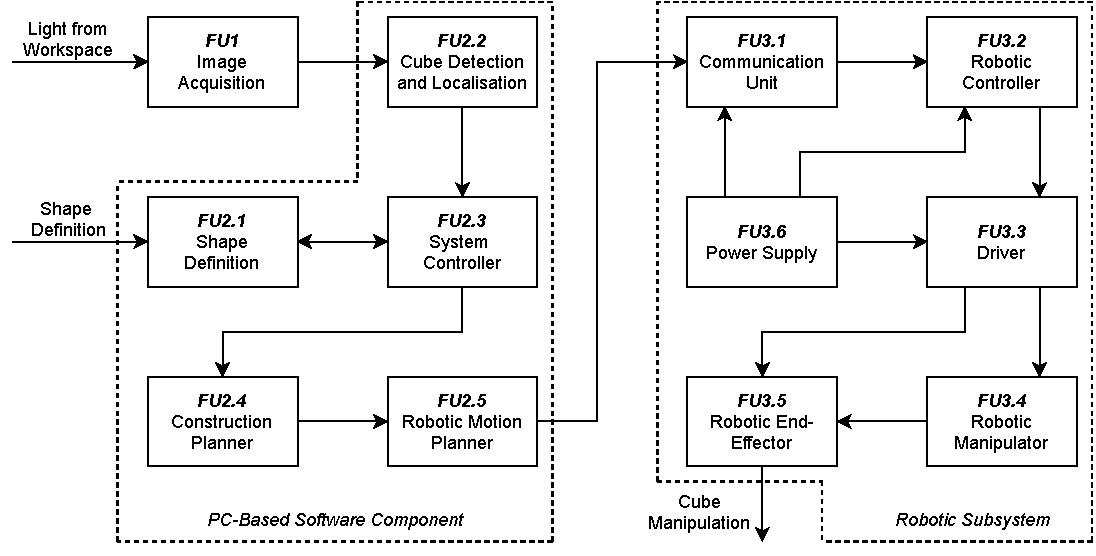
\includegraphics[width=0.8\linewidth]{figures/functional-block-diagram.pdf}
  \caption{Block diagram showing the proposed functional structure of the system.}
  \label{fig:functional_block_diagram}
\end{figure}

\pendsign

\section[2021/04/21]{Wednesday, 21 April 2021}

\subsection{PC-Based Software selection}

C++ was selected as the protoytyping programming language to be used for the development of the PC-based software components. These include the cube detection, robotic localisation, shape definition \ac{GUI}, construction planner and robotic path planner components. The primary criteria for the selection of C++ was its better performance compared to Python which is also frequently used in the context of computer vision. Python is suitable when using computer vision libraries since they are usually implemented in C or C++ and called using a python wrapper to still enjoy great performance. However, since this project requires the implementation of the functions of these libraries from scratch, it is more efficient to code the algorithms from first principles in C++. C++ was selected to implement the \ac{GUI} as well since the majority of the computational code will already be written in C++ and it also makes integration between the different components of the PC-based software less complex. QT framework was selected to implement the \ac{GUI} component as it is the market leader in this field for the C++ programming language and has excellent support for integration with a graphic \ac{API}.

\pendsign

\section[2021/04/24]{Saturday, 24 April 2021}

\subsection{Literature Review: An Introductory Guide to Computer Vision \cite{tryolabs_resources_2019}}

Computer vision is related to image processing and machine vision. The primary focus of image processsing is the application of transformations to raw images while machine vision is a special case of computer vision in production environments where it is used to perform actions. Computer vision is used to solve more complex problems such as object recognition. Image classification, localisation, object detection, object identification, instance segmentation and object tracking are typical computer vision tasks. The Viola and Jones algorithm has been one of the most popular approaches to object detection challenges. A \ac{CNN} is a modern deep learning tool that has achieved excellent results using traditional computer vision methods.

\subsection{Literature Review: Robotic Object Recognition and Grasping with a Natural Background \cite{Wei2020}}

The following important terms are used in the article:

\begin{compactitem}
    \item \textit{Grasp synthesis} entails finding a grasp configuration that complies with a set of criteria for a given grasping task.
    \item A \textit{superpixel} is collection of pixels that are related by similar characteristics.
    \item The \textit{\ac{MTCD}} is a contour-based shape descriptor that extracts triangles from each contour point. \cite{Yang2016}
\end{compactitem}

Factors that provide uncertainty with object recognition are illumination, occlusion, and the pose of the object. There are generally two main methods for robot grasping, namely empirical methods and analytical methods. Deep-learning techniques have found popularity more recently in this field. The general deep-learning strategy involves identifying the object to be grasped from the image from a series of candidates which are ranked using a \ac{CNN} before grasping the selected candidate in an open-loop fashion. The following disadvantages are presented by the \ac{CNN} deep-learning based approach:

\begin{compactitem}
    \item Precise end-effector and and camera calibration is required.
    \item A large annotated dataset is required for training and testing.
    \item The \ac{CNN} models may lack the ability to generalise well.
    \item The processing time to rank potential objects using the \ac{CNN} may take too much time.
    \item The localisation of objects is only course which is not suited to precision tasks.
\end{compactitem}

Superpixel segmentation can be used to group pixels into distinct regions that have perceptual meaning and provides noise suppression. This article presents a solution that combines superpixel segmentation and edge detection to attain true contour information from the image objects. The algorithm uses this contour information along with the \ac{MTCD} shape descriptor and shape dissimilatiry information as heuristics to guide comparison of contours to exisiting object contours in a reasonable amount of time.

\pendsign